\chapter{Aplicaciones}
\section{Maniobra y protección de motores}
Los defectos de en motores se clasifican en:
\begin{itemize}
	\item Sobrecargas térmicas (50 \%)
	\begin{itemize}
		\item Causas mecánicas
		\begin{itemize}
			\item Aumento anormal del par resistente
			\item
			Bloqueo del rotor
			\item
			Arranques lentos
		\end{itemize}
		\item Causas eléctricas
		\begin{itemize}
			\item Fallo de fase
			\item
			Desequilibrio
			\item
			Subtensión
			\item
			Sobretensión
		\end{itemize}
		\item Otras causas
		\begin{itemize}
			\item Temperatura ambiente excesiva
			\item
			Fallo de la refrigeración
			\item
			Servicio intermitente inadmisible
		\end{itemize}
	\end{itemize}
	\item Cortocircuitos (40\%), causados por defectos de aislamiento provocados por:
	\begin{itemize}
		\item Humedad
	\item
		Polvo
		\item
		Grasa
		\item
		Productos químicos
	\item
		Daños mecánicos 
	\end{itemize}
	
\end{itemize}
\subsection{Arrancador}
Se define como el conjunto de dispositivos que permiten abrir y cerrar el circuito de conexión a la red y proteger el motor. Tiene las siguientes funciones:
\begin{itemize}
	\item Protección frente cortocircuitos
	\item Protección contra sobrecargas
	\item Seccionamiento
	\item Mando de potencia
\end{itemize}

Para ello, se emplean relés especiales cuyo número de clase representa el tiempo de disparo máximo permitido en segundos para una corriente 7,2 veces la asignada.
\begin{itemize}
	\item Clase 10A y clase 10: arranque normal
	\item Clase 20 y 30: arranque fuerte
\end{itemize}

Estos arrancadores están formados por alguno de los siguientes elementos:
\begin{itemize}
	\item \textbf{Fusible + seccionador o interruptor automático}: protección contra cortocircuitos y seccionamiento del circuito
	\item \textbf{Relé térmico}: protege frente a sobrecargas y falta de fase
	\item \textbf{Contactor}: tiene como objetivo la maniobra y apertura por acción del relé térmico
\end{itemize}
\subsection{Coordinación en un arrancador}
\begin{itemize}
	\item Tipo 1:
	\begin{itemize}
		\item Se permite un cierto deterioro del contactor en caso de cortocircuito
		\item
		Coste aparamentabajo y requiere mantenimiento
	\end{itemize}
	\item Tipo 2:
	\begin{itemize}
		\item No se admite ningún deterioro del contactor en caso de cortocircuito
		\item
		Mayor coste de la aparamentay menor necesidad de mantenimiento
	\end{itemize}
\end{itemize}
\subsection{Tipo de interruptor automático en función de la potencia}
\begin{itemize}
	\item $P_m<250,kW$: Caja moldeada
	\item $250,kW,<P_mz<630,kW$: Bastidor abierto
	\item $P_m>630,kW$: Alimentación en media tensión
\end{itemize}
\section{Protección de generadores}
Se debe tener en cuenta si las cargas están alimentadas por el generador y la red simultáneamente o no para poder dimensionar adecuadamente los poderes de corte. Se habla de alimentación alternativa si se da que mediante un sistema de conmutación se impida el acoplamiento simultáneo a ambas fuentes de alimentación.
\newline

La transferencia de carga entre red y generador puede ocurrir de dos maneras:
\begin{enumerate}
	\item Con corte de tensión
	\item Sin corte de tensión: obliga a equipo de sincronización, sólo para generadores con potencia superior a 100 kVA
\end{enumerate}

En locales de pública concurrencia la conmutación entre el suministro normal y el de seguridad debe realizarse de forma que se impida el acoplamiento entre ambos suministros.
\newline

A continuación, se muestra el ejemplo de un cuadro con grupos electrógenos.
\begin{figure}[H]
	\centering
	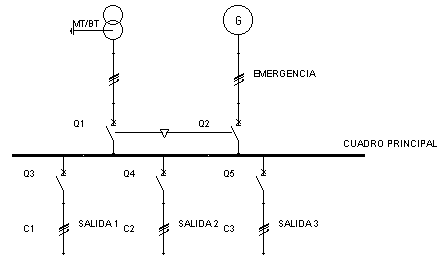
\includegraphics[width=0.7\linewidth]{Images/21}
\end{figure}

Para el cálculo del cortocircuito en bornes del generador se usa la siguiente expresión donde $ X_d''(\%)$ es la impedancia subtransitoria:
\begin{equation}
	I''=\dfrac{I_N}{X_d''(\%)} \rightarrow I_N=\dfrac{S_N}{\sqrt{3}U_N}
\end{equation}

Para garantizar la selectividad (si ha entrado el grupo electrógeno es normalmente es importante que no se caiga toda la instalación) se debe cumplir que el disparo instantáneo en el grupo de emergencia sea:
\begin{equation}
	I_{mQ2}> 1,5 max(I_{mQi})
\end{equation}

Como no siempre es posible asegurar selectividad en la zona térmica se emplean relés de prestaciones especiales con un ajuste distinto para tensión de red y de alimentación por el grupo electrógeno.
\section{Sistemas de alimentación ininterrumpida SAI}
Impiden que las cargas prioritarias o criticas pasen por cero en caso de conmutación red-grupo. Alimentan las cargas durante un tiempo determinado en caso de ausencia de alimentación de red y de grupo. 
\newline

Normalmente los cuadros con una SAI tienen un esquema unifilar similar al presentado a continuación (el bypass manual es para mantenimiento):
\begin{figure}[H]
	\centering
	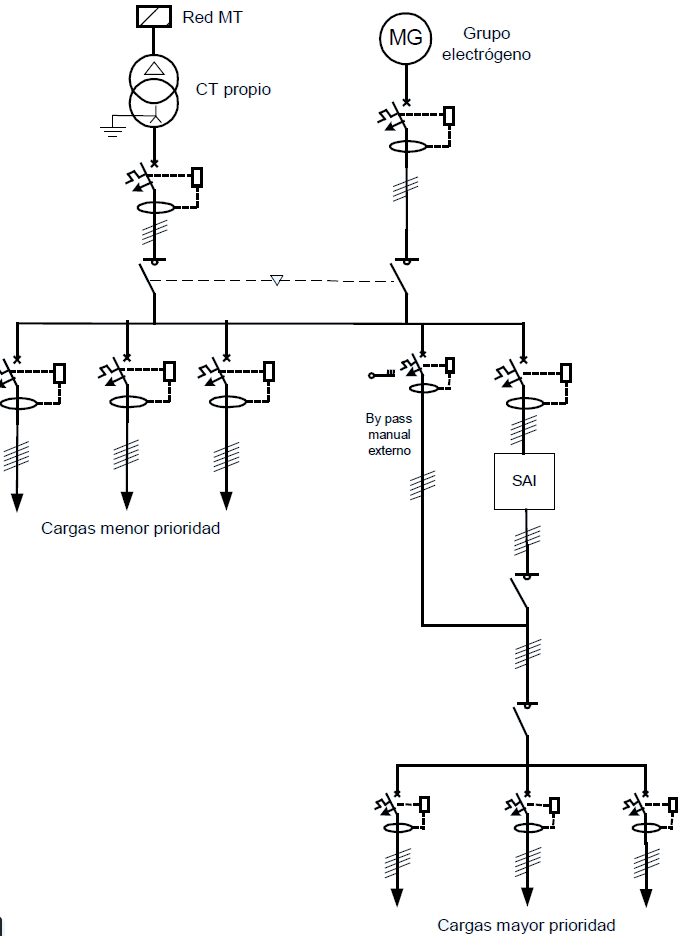
\includegraphics[width=0.7\linewidth]{Images/22}
\end{figure}

\subsection{Modos funcionamiento SAI}
\begin{itemize}
	\item \textbf{Normal}: tensión de red o de grupo.
	La carga es alimentada por la red a través del SAI
\item
	\textbf{Emergencia}: sin tensión red ni de grupo.
	La carga es alimentada por la batería y el inversor
\item
	\textbf{Sobreintensidad temporal}: arranque motor.w
	Alimentación por la red a través de by-passelectrónico interno
	\item
	\textbf{Mantenimiento SAI}:
	La carga es alimentada por la red a través de by-passmanual externo
	
	

\end{itemize}
\subsection{SAI en estado de emergencia y sobreintensidad}
Las sobrecargas cuando alimenta la SAI son asumidas por la batería y tiene las siguientes características Intensidad-tiempo:
\begin{table}[H]
	\centering
	\begin{tabular}{|c|c|}
		\hline
		\textbf{I}            & \textbf{Tiempo (s)} \\ \hline
		$1,15\times I_n$           & $\infty$                               \\ \hline
		$1,25\times I_n$             & 600                                \\ \hline
		$1,5\times I_n$              & 60                                \\ \hline
		$2\times I_n$              & 1                              \\ \hline
	\end{tabular}
\end{table}

En cuanto al cortocircuito se considera que la SAI puede aportar el 200\% del valor nominal de la corriente.
\newline

En estos estados se debería establecerse selectividad entre los interruptores automáticos aguas abajo del SAI y el inversor, lo que es difícil.
\section{Protección de condensadores}
Primero se debe calcular la intensidad nominal de los condensadores:
\begin{equation}
	I_{NC}=\dfrac{Q_N}{\sqrt{3}U}
\end{equation}

Para seleccionar la intensidad nominal del interruptor, $I_{NQ}$, se sigue el siguiente criterio:
\begin{equation}
	I_{NQ}> 1,5 I_{NC} 
\end{equation}

En cuanto a los ajustes del relé magnético se debe tener en cuenta que la conexión de una batería de condensadores es comparable a un cierre de cortocircuito \textbf{(corrientes elevadas de corta duración)}.
\newline

Para relés magnetotérmicos:
\begin{equation}
	I_{mNDQ}>10 I_{NC}
\end{equation}

Para relés electrónicos se debe desactivar la protección instantánea frente a cortocircuitos
\section{Alimentación por varios transformadores en paralelo}
Se debe tener en cuenta que como son impedancias en paralelo la corriente de cortocircuito aumenta y se da el caso de que los interruptores a la salida de los transformadores requieren menor poder de corte que los de entrada a las líneas aguas abajo.